\documentclass{article}
\usepackage[left=2cm, right=5cm, top=2cm]{geometry} 
\usepackage{graphicx}
%\documentclass[a4paper,10pt]{scrartcl}

\usepackage[utf8]{inputenc}

\title{Sílabus: Samba de Gafieira - Nível I}
\author{Fernando Pujaico Rivera}
\date{}

\pdfinfo{%
  /Title    (Sílabus: Samba de Gafieira - Nível I )
  /Author   (Fernando Pujaico Rivera)
  /Creator  ()
  /Producer ()
  /Subject  ()
  /Keywords (Samba, Gafieira)
}


\begin{document}
{\let\newpage\relax\maketitle}
A Tabela \ref{tab:typospos} e \ref {tab:typosmov}, descrevem a notação de nomes  (posturas e movimentos) usadas 
na descrição do programa de aula.
A Figura \ref{fig:mov} mostra como são relacionados as posturas e os distintos tipos de movimentos.


\begin{table}[h]
\centering
\begin{tabular}{|p{3cm}|p{13cm}|}
\hline
~ & Descrição \\  \hline
Postura & No transcurso das aulas, chamaremos postura o pose, a una distribuição estática
dos membros do corpo. Uma postura estabelece um ponto de inicio para a execução de um
movimento; assim, um movimento inicia e termina sempre numa postura o pose.\\ \hline

\end{tabular}
\caption{Descrição de uma postura}
\label{tab:typospos}
\end{table}


\begin{table}[h]
\centering
\begin{tabular}{|p{3cm}|p{13cm}|}
\hline
Movimento & Descrição \\  \hline
\textbf{Passo (básico)} & Movimento de nível iniciante; o conhecimento deste 
movimento é necessário para enlaçar/interconectar movimentos mais complexos ensinados nas aulas. Estes
movimentos tem uma característica cíclica, é dizer, a postura do final do movimento 
é igual à postura de inicio. Os passos básicos são: Frente e trás (F.T.), Balanço e Cruzado.\\ \hline
\textbf{Passo} &  Movimento genérico com uma execução com uma amplitude de dificuldade desde simples a complexo.
Um passo inicia e termina numa postura, a qual pode ser a mesma. Definiremos um passo, como um movimento
notável, pelo qual este tem ganhado um nome própio; exemplo: Gatilho, Gancho redondo, Puladinho, Tesoura, etc. \\ \hline
\textbf{Transição ou movimento de transição} &  Movimento extremadamente simples, pelo qual não tem nome própio,
e consta de poucas transições. Exemplo: transição entre Frente trás e o Balanço, ou a transição entre Balanço e o Cruzado.\\ \hline
\end{tabular}
\caption{Tipos de movimentos.}
\label{tab:typosmov}
\end{table}



\begin{figure}[h]
  \centering
  \caption{ Movimento sendo executado desde uma postura ate outra postura.}
  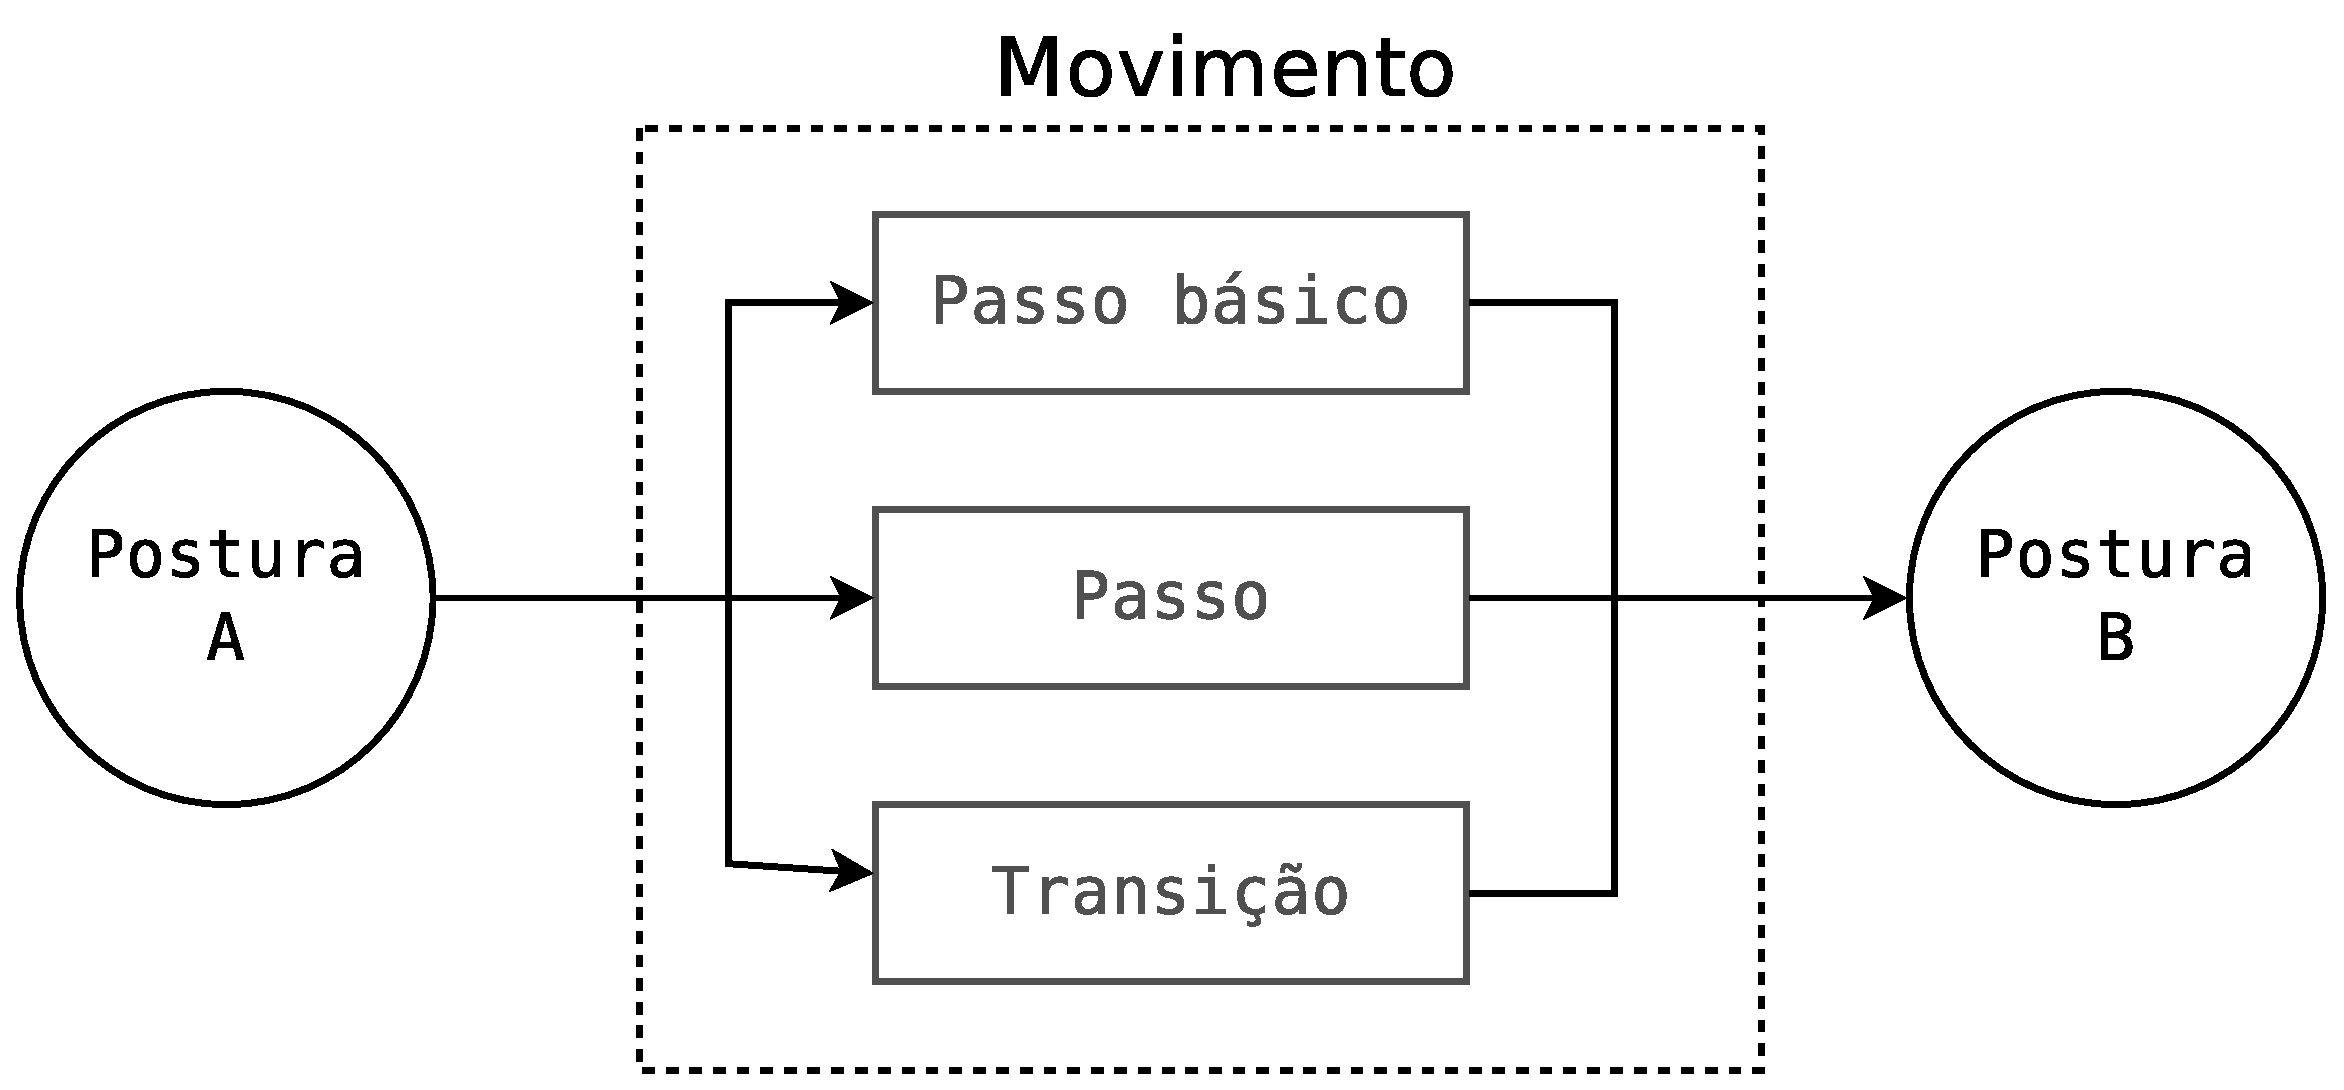
\includegraphics[width=0.8\textwidth]{Diagrama1.eps}% picture filename
  \label{fig:mov}
\end{figure}



A Tabela \ref{tab:myfirsttable} mostra a descrição do conteúdo das aulas de samba de gafieira.


\begin{table}[h]
\centering
\begin{tabular}{|p{1.5cm}|p{5cm}|p{9cm}|}
\hline
Semana & Tema & Descrição \\  \hline
1 &  \textbf{Passos básicos:} Frente e trás (F.T.) e Balanço & Serão estudados os movimentos de transição entre o balaço e F.T. e enfeites no giro do balanço.\\ \hline
2 &  \textbf{Passo básico:} Cruzado &  Serão estudados os movimentos de transição entre o balaço e o cruzado, e enfeites no cruzado. \\ \hline
3 &  \textbf{Transição:} Saída lateral. &  Serão estudados o movimentos de transição entre F.T. e cruzado e enfeites na saída lateral.\\ \hline
4 &  \textbf{Transição:} gancho. \textbf{Postura:} X &  Serão estudados os movimentos de transição entre cruzado e F.T., além das posturas notáveis.\\ \hline                     
5 &  \textbf{Passo:} Gatilho &  Serão estudados os movimentos de transição entre F.T. e cruzado. \\ \hline
5 &  \textbf{Passo:} Edmundo &  Serão estudados o controle de equilíbrio e eixo do corpo. \\ \hline
6 &  \textbf{Passo:} Caminhada em contratempo & Será estudado a distribuição de tempos na caminhada em contratempo. \\ \hline
6 &  \textbf{Passo:} Sacada de perna & Será estudado a sacada de perna de ambos. \\ \hline
7 &  \textbf{Passo:} Facão, \textbf{Postura}: Facão & Será estudado dois estilos de facão (movimento discreto e ondulado) e a postura de finalização. \\ \hline
8 &  \textbf{Passo:} Puladinho & Será estudado a consciência corporal necessária para executar o movimento, adicionalmente será agregado um enfeite para o movimento. \\ \hline
9 &  \textbf{Passo:} Romário & Será estudado a condução, postura do corpo e eixo para a execução do movimento, adicionalmente serão agregados dois enfeites para o movimento. \\ \hline
10&  \textbf{Passo:} Assalto & Será estudado a diferença entre Assalto e Bailarina, adicionalmente serão estudados enfeites de mãos para o movimento. \\ \hline
11&  \textbf{Passo:} Escovinha desde caminhada & Será iniciado o estudo dos movimentos de la família da escovinha. \\ \hline

\end{tabular}
\caption{Descrição do conteúdo}
\label{tab:myfirsttable}
\end{table}

\end{document}
